\begin{frame}
    \vspace*{0.5in}
    \begin{center}
        \Large \textbf{Example Application}: Hypersonic Thermal Protection Systems
    \end{center}
    \begin{figure}
        \vspace*{-0.2in}
        \centering
        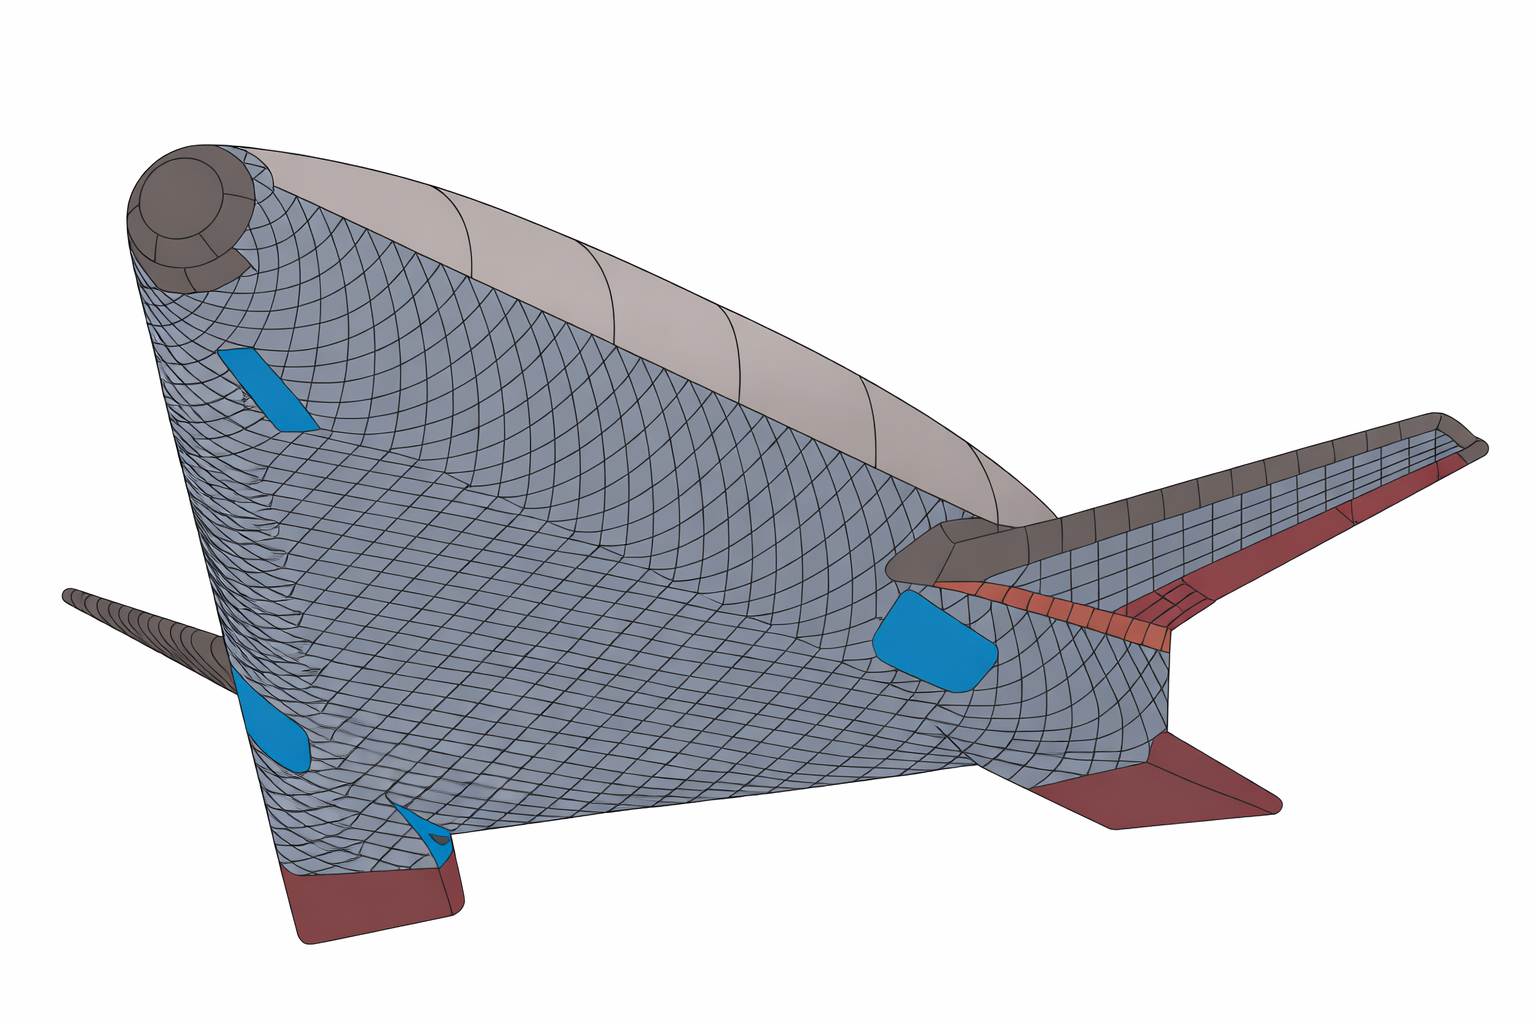
\includegraphics[width=0.5\textwidth]{../figs/tps/tps_vehicle.png}
    \end{figure}
\end{frame}

\begin{frame}{\small The formulation starts with \textbf{model-order reduction},}
    \footnotesize
    \begin{columns}
        \visible<2->{
        \begin{column}{0.35\textwidth}
                \centering
                \textbf{Full-Order Model} (e.g., FEM)
                \begin{align*}
                    \dot{\vx} &= \vF\left(\vx;\vp\right)\\
                    \vz_{\text{HF}} &= \vH\left(\vx;\vp\right)\\
                    \vx(t_0) &= \vx_0
                \end{align*}
                \vspace{-0.2in}
                \begin{enumerate}
                    \item<3-> $\vx\in\mathbb{R}^{n_x}$: states $(n_x\gg 1)$
                    \item<4-> $\vp\in\mathbb{R}^{n_p}$: parameters
                    \item<5-> $\vz_{\text{HF}}\in\mathbb{R}^{n_z}$: QoI 
                \end{enumerate}
        \end{column}}
        \visible<6->{
        \begin{column}{0.70\textwidth}
            \centering
            \textbf{Coarse Graining} (reduce FOM's complexity)
            \begin{enumerate}
                \item<7-> State decomposition $\vx = \left[\bvx,\deltavx\right]^{\top}\in\mathbb{R}^{n_x}$ 
                \begin{itemize}
                    \item<8-> Averaging variables (observables) $\bvx\in\mathbb{R}^{n_{\bar{x}}}$
                    \item<9-> Un-resolved (un-observables) $\deltavx\in\mathbb{R}^{n_{\delta x}}$ $\left(n_{\delta x}\gg n_{\bar{x}}\right)$
                \end{itemize}
                \item<10-> Projection operator $\cP:\cH_{n_x}\to\cH_{n_{\bar{x}}}\subset\cH_{n_x}$, e.g.,
                \vspace*{-0.1in}
                \begin{equation*}
                    \cP: \cG\left(\vx\right)\rightarrow \bar{\cG}\left(\bvx\right)\rightarrow\text{\textbf{cheaper to evaluate!}}
                    \vspace*{-0.1in}
                \end{equation*}
                \item<11-> Complement operator $\cQ = \cI - \cP$
            \end{enumerate}
            \vspace{-0.1in}
            \visible<12->{
            \begin{figure}
                \centering
                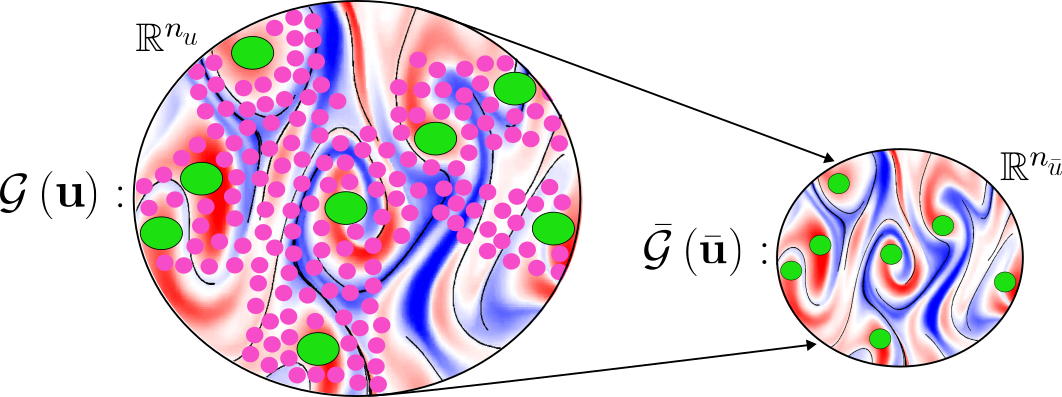
\includegraphics[width=0.7\textwidth]{../figs/pirom/coarse_graining.png}
            \end{figure}}
        \end{column}}
    \end{columns}
\end{frame}

\begin{frame}{\small For example, \textbf{coarse-graining} the TPS proceeds as follows,}
    \footnotesize
    \vspace*{-0.2in}
    \begin{columns}
        \visible<1->{
        \begin{column}{0.55\textwidth}
            \only<1>{
                \begin{figure}
                    \centering
                    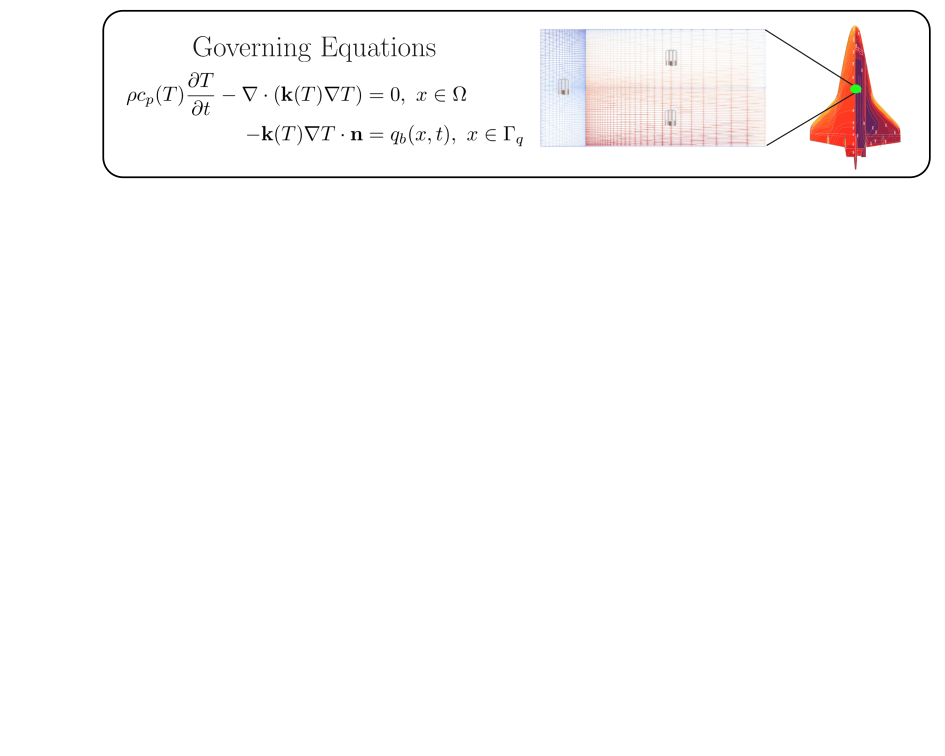
\includegraphics[width=0.85\textwidth]{../figs/pirom/coarse_graining_tps_left_1.png}
                \end{figure}}
            \only<2>{
                \begin{figure}
                    \centering
                    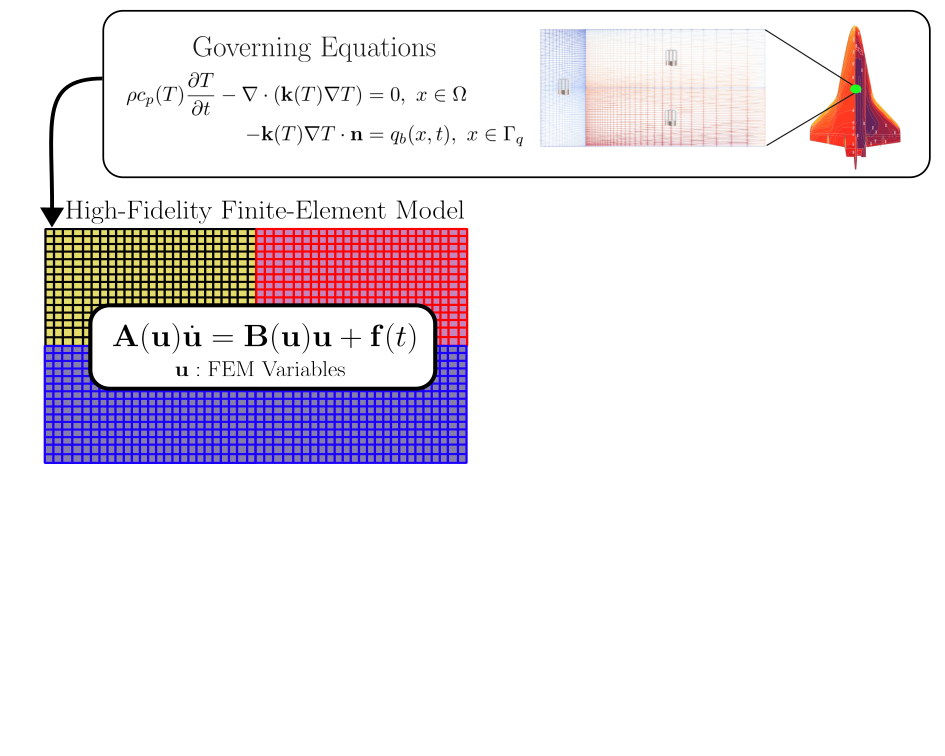
\includegraphics[width=0.85\textwidth]{../figs/pirom/coarse_graining_tps_left_2.png}
                \end{figure}}
            \only<3>{
                \begin{figure}
                    \centering
                    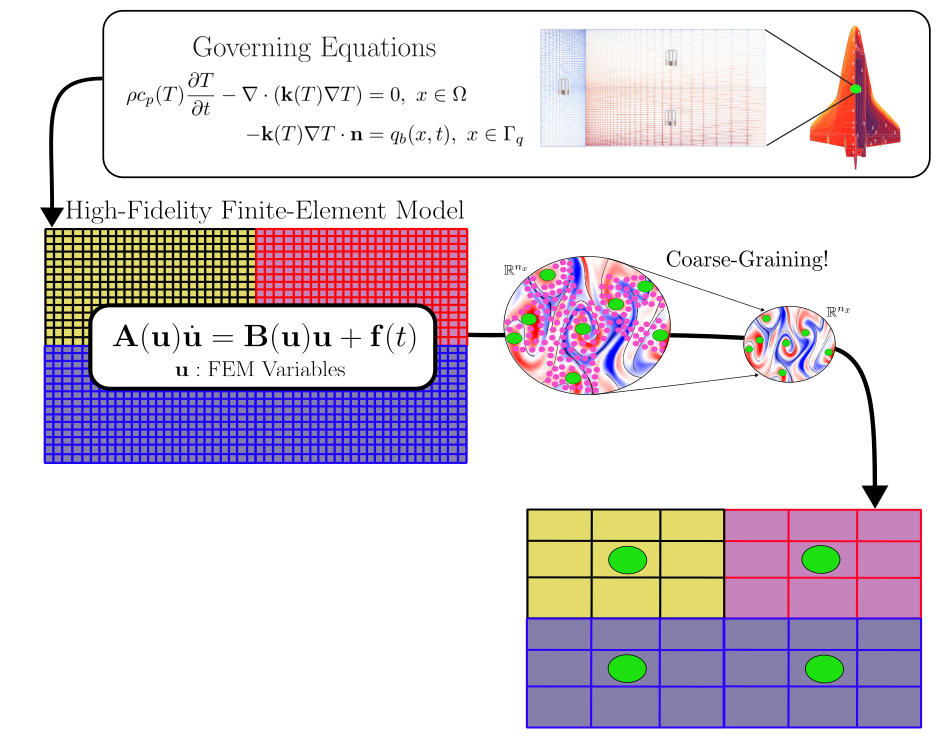
\includegraphics[width=0.85\textwidth]{../figs/pirom/coarse_graining_tps_left_3.png}
                \end{figure}}
            \only<4->{
                \begin{figure}
                    \centering
                    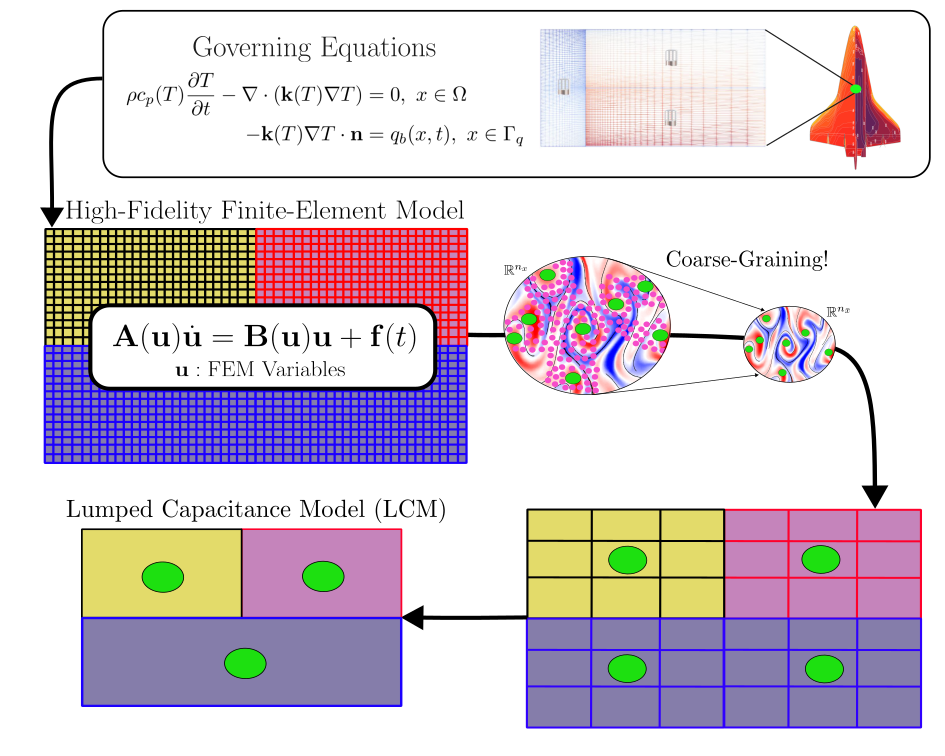
\includegraphics[width=0.85\textwidth]{../figs/pirom/coarse_graining_tps_left_4.png}
                \end{figure}}
        \end{column}}
        \hspace*{-0.25in}
        \visible<1->{
        \begin{column}{0.55\textwidth}
            \vspace*{-0.05in}
            \only<5>{
                \begin{figure}
                    \centering
                    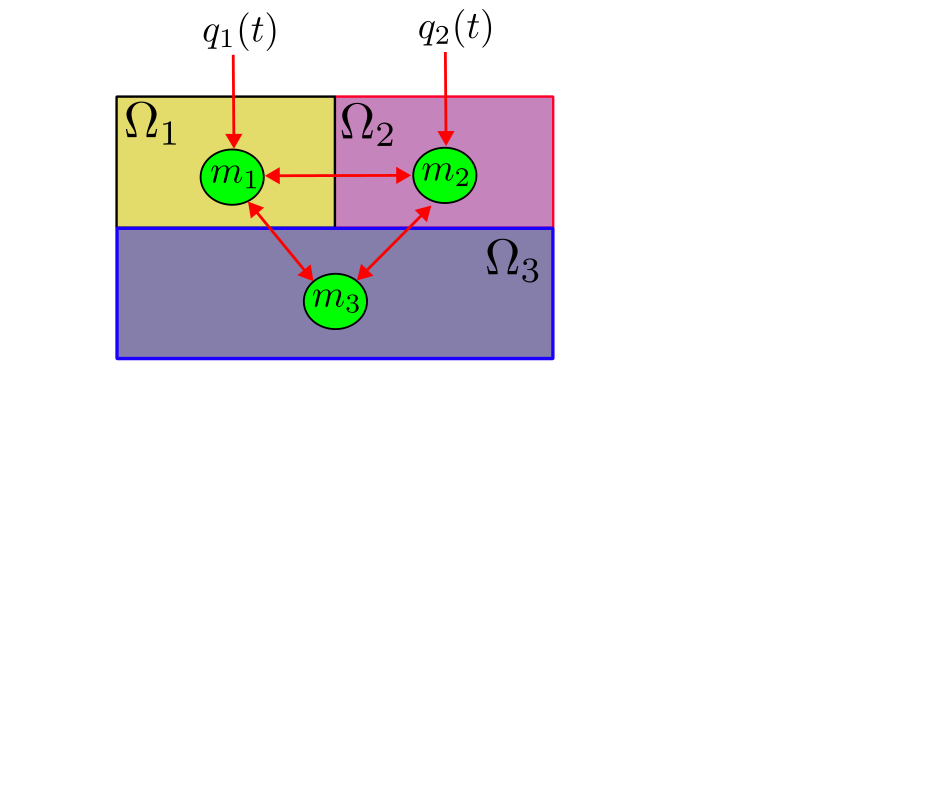
\includegraphics[width=0.95\textwidth]{../figs/pirom/coarse_grained_variables_tps_1.png}
                \end{figure}}
            \only<6>{
                \begin{figure}
                    \centering
                    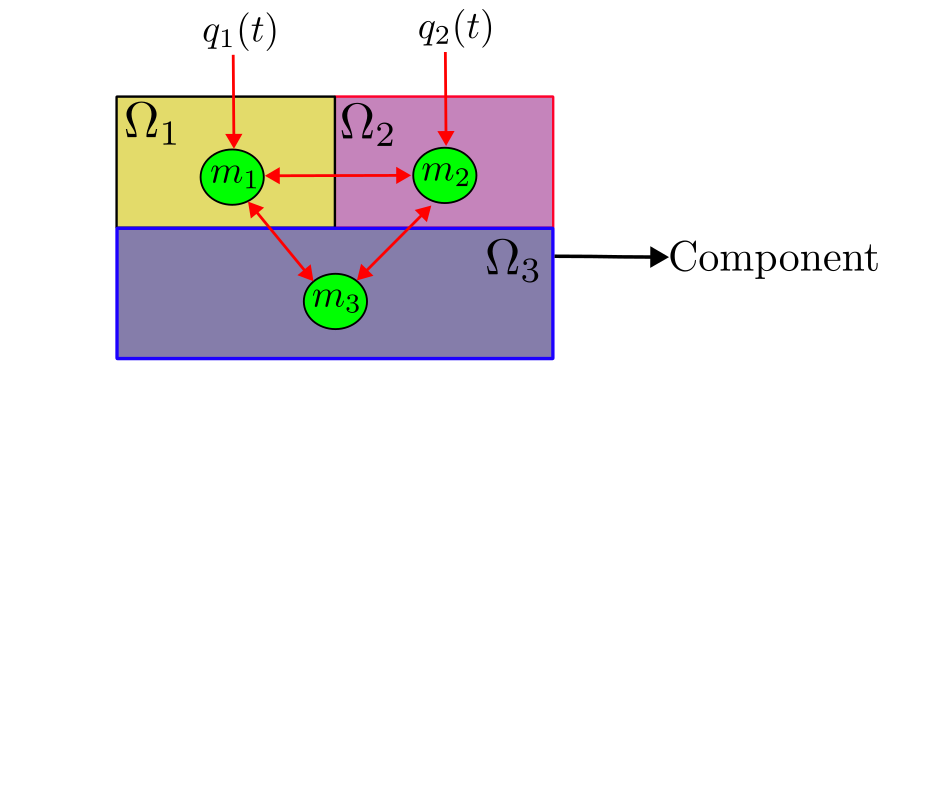
\includegraphics[width=0.95\textwidth]{../figs/pirom/coarse_grained_variables_tps_2.png}
                \end{figure}}
            \only<7>{
                \begin{figure}
                    \centering
                    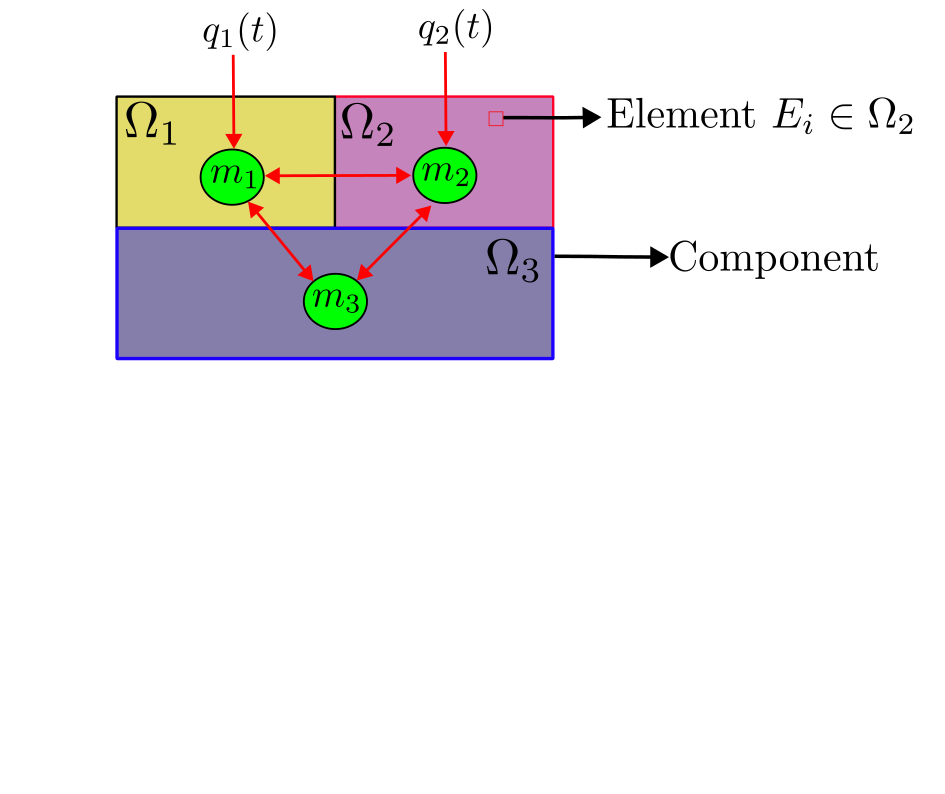
\includegraphics[width=0.95\textwidth]{../figs/pirom/coarse_grained_variables_tps_3.png}
                \end{figure}}
            \only<8>{
                \begin{figure}
                    \centering
                    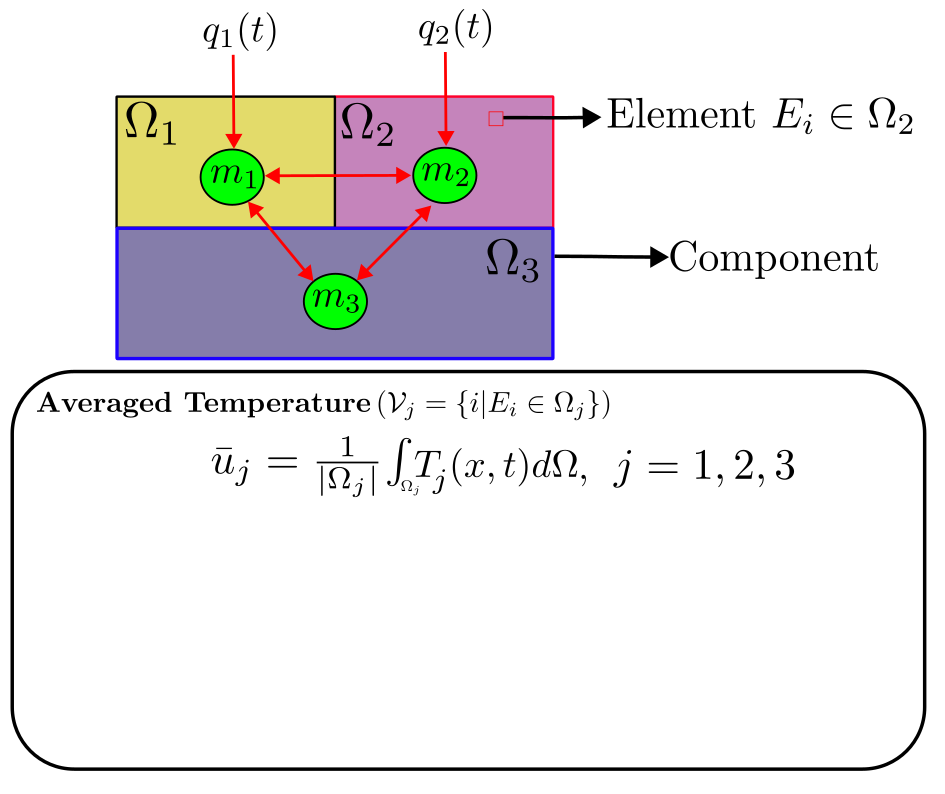
\includegraphics[width=0.95\textwidth]{../figs/pirom/coarse_grained_variables_tps_4.png}
                \end{figure}}
            \only<9>{
                \begin{figure}
                    \centering
                    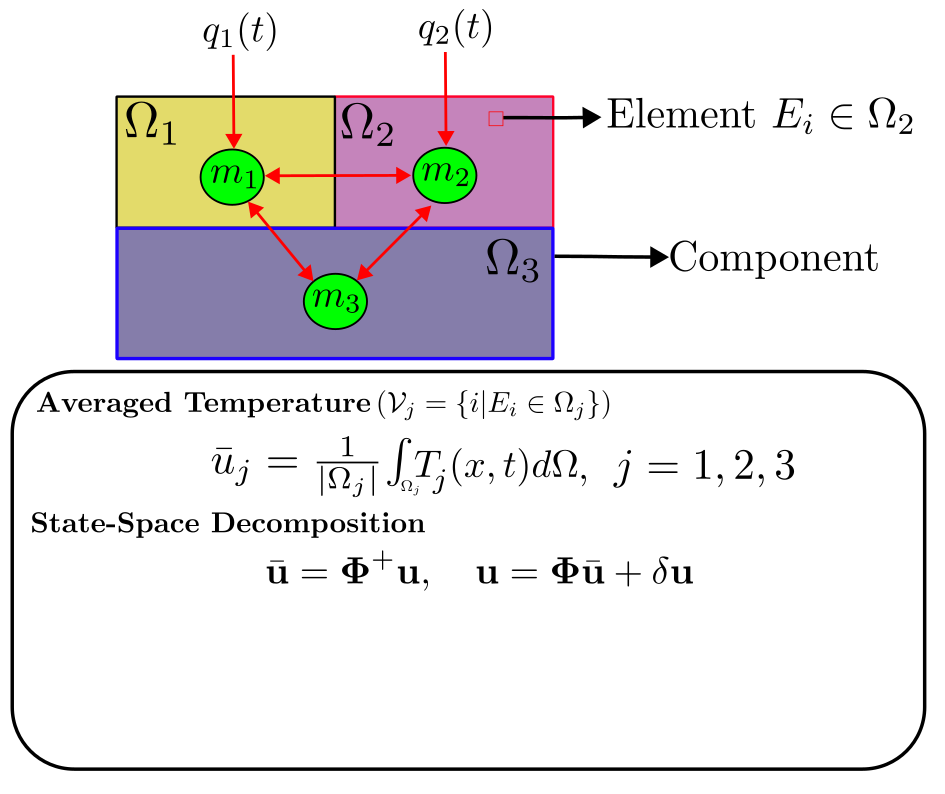
\includegraphics[width=0.95\textwidth]{../figs/pirom/coarse_grained_variables_tps_5.png}
                \end{figure}}
            \only<10>{
                \begin{figure}
                    \centering
                    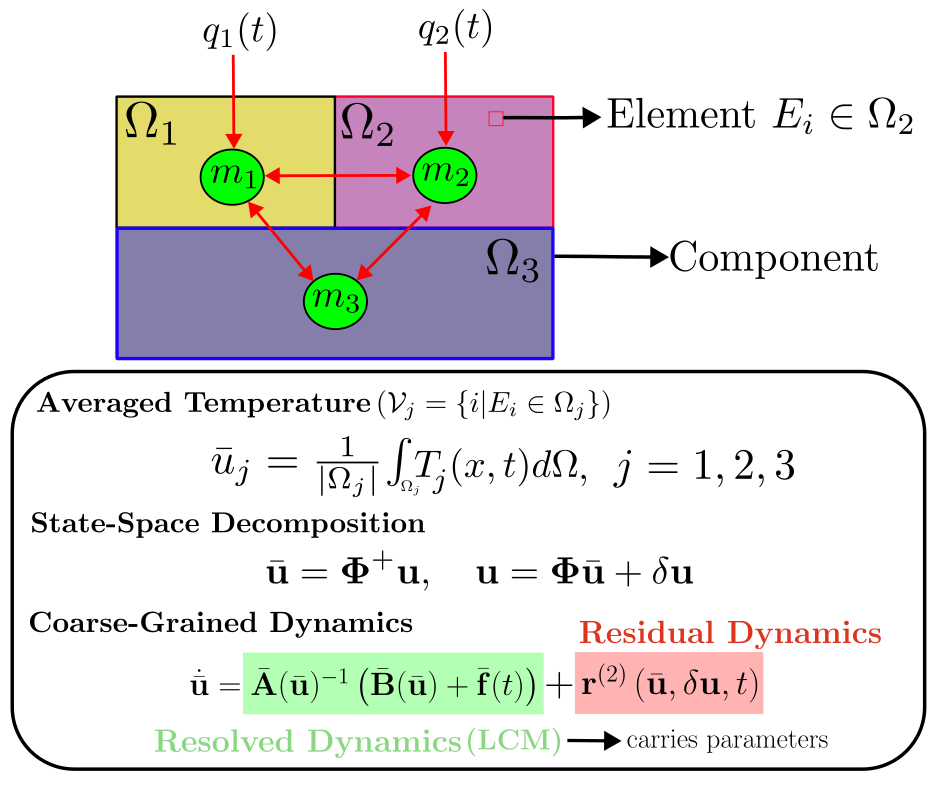
\includegraphics[width=0.95\textwidth]{../figs/pirom/coarse_grained_variables_tps_6.png}
                \end{figure}}
        \end{column}}
    \end{columns}
\end{frame}

\begin{frame}{\small We need to \textbf{efficiently model} the \textbf{residual dynamics},}
    \footnotesize
    \vspace*{-0.3in}
    \begin{equation*}
        \text{Projected GLE}:\quad \underbrace{\frac{\partial}{\partial t} \cP e^{t\cL}\bvu}_{\text{Observable Dynamics}} \visible<3->{= \underbrace{\cP e^{t\cL}\cP\cL\bvu}_{\text{Markovian}}} \visible<4->{+ \cP\underbrace{\int_0^t e^{(t-s)\cL}\cP\cL e^{s\cQ\cL}\cQ\cL\bvu ds}_{\text{Non-Markovian}}} \visible<5->{+ \cP\underbrace{e^{t\cQ\cL}\cQ\cL\bvu}_{\text{Noise}}}
    \end{equation*}
    \begin{columns}
        \visible<3->{
        \begin{column}{0.3\textwidth}
            \centering
            \textbf{Markovian}
            \begin{figure}
                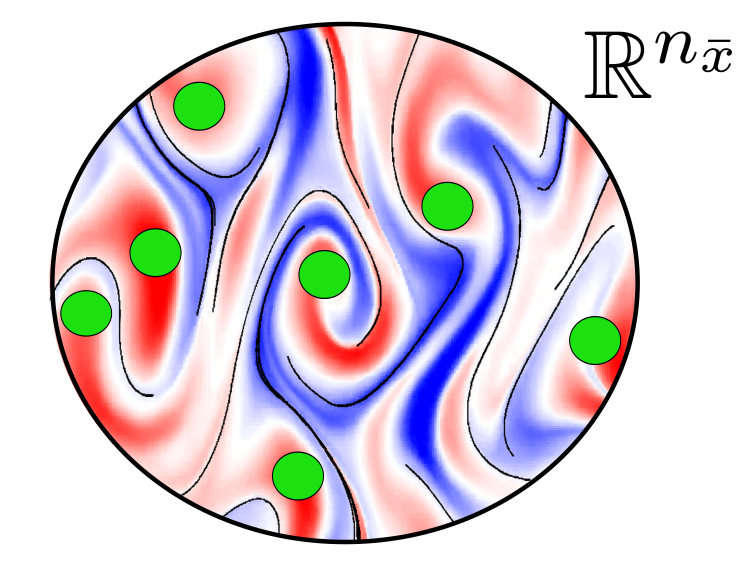
\includegraphics[width=0.9\textwidth]{../figs/pirom/coarse_variables.png}
            \end{figure}
            {\small (known dynamics)}
        \end{column}}
        \visible<4->{
        \begin{column}{0.3\textwidth}
            \centering
            \textbf{Non-Markovian}
            \begin{figure}
                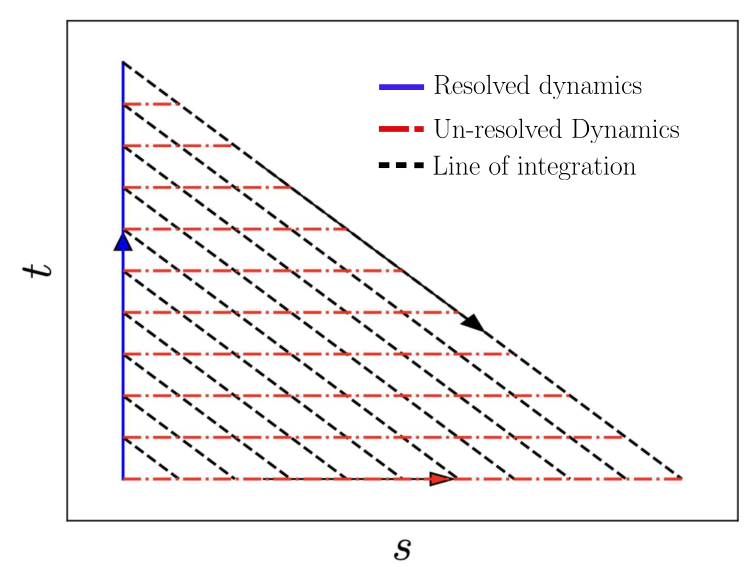
\includegraphics[width=0.9\textwidth]{../figs/pirom/memory.png}{\tiny [1]}
            \end{figure}
            {\small\textcolor{red}{(unknown dynamics)}}
        \end{column}}
        \visible<5->{
        \begin{column}{0.3\textwidth}
            \centering
            \textbf{Noise}
            \begin{figure}
                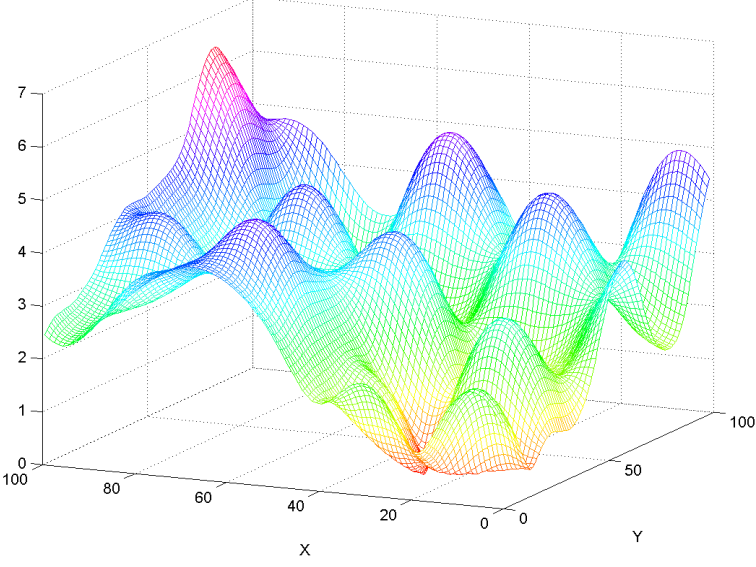
\includegraphics[width=0.9\textwidth]{../figs/pirom/noise.png}
            \end{figure}
            {\small\textcolor{black}{(orthogonal to $\cP$)}}
        \end{column}}
    \end{columns}
    \begin{center}
    {\tiny GLE: Generalized Langevin Equation, $\cL$: Liouville operator, PGLE: Projected GLE}
    \end{center}
\end{frame}

\begin{frame}{\small\textbf{Physics infusion} is performed as follows,}
    \footnotesize
    \vspace*{-0.3in}
    \begin{columns}
        \begin{column}{0.5\textwidth}
            \begin{center}
                \textbf{Memory Kernel Approximation}
            \end{center}
                \visible<3->{
                Define the memory kernel,
                \begin{equation*}
                    \vkappa(\bvu,t,s) = \cP e^{(t-s)\cL}\cP\cL e^{s\cQ\cL}\cQ\cL\bvu
                \end{equation*}}
                \visible<4->{
                Parametrize the \textbf{memory kernel},
                \begin{equation*}
                    \vkappa(\bvu,t,s;\redvTheta) \approx \sum_{j=1}^{m} \cK_j(t,s,\bvu;\redvTheta)\phi_j(s,\bvu;\redvTheta)
                \end{equation*}}
                \visible<5->{
                For \textbf{TPS problem}, design $\cK_j$ and $\phi_j$ as,
                \begin{align*}
                    \cK_j(t,s,\bvu;\redvTheta) &= e^{-\textcolor{red}{\lambda_j}(t-s)}\Rightarrow\text{{\tiny \textbf{exponential decay!}}}\\
                    \phi_j(s,\bvu;\redvTheta) &= \textcolor{red}{\vp_j}\left(\textcolor{red}{\vq_j}^\top\bar{\vu}(s) + \textcolor{red}{\vr_j}^\top\underbrace{\bar{\vf}(s)}_{\text{external forcing}} \right)
                \end{align*}}
        \end{column}
        \hspace*{-0.1in}
        \begin{column}{0.55\textwidth}
            \begin{center}
                \textbf{Markovian Reformulation}
            \end{center}
                \visible<7->{
                Define the memory variable as,
                \begin{equation*}
                    \beta_j(t) = \int_0^t e^{-\textcolor{red}{\lambda_j}(t-s)} \left(\textcolor{red}{\vq_j}^\top\bar{\vu}(s) + \textcolor{red}{\vr_j}^\top\bar{\vf}(s)\right) ds
                \end{equation*}}
                \visible<8->{
                so that the hidden dynamics are,
                \begin{equation*}
                    \dot{\beta}_j = \textcolor{red}{\lambda_j}\beta_j + \textcolor{red}{\vq_j}^\top\bar{\vu} + \textcolor{red}{\vr_j}^\top\bar{\vf},\:\: j=1,\dots,m
                \end{equation*}}
                \visible<9->{
                Thus, the PIROM is written as,
                \begin{align*}
                    \dot{\bvu} &= \underbrace{\cP e^{t\cL}\cP\cL\bvu}_{\text{\textbf{LCM dynamics!}}} + \sum_{j=1}^{m}\textcolor{red}{\vp_j}\beta_j\\
                    \dot{\beta}_j &= \textcolor{red}{\lambda_j}\beta_j + \textcolor{red}{\vq_j}^\top\bar{\vu} + \textcolor{red}{\vr_j}^\top\bar{\vf}\\
                    \vz &= \textcolor{red}{\vD_{\bar{u}}}\bvu + \textcolor{red}{\vD_{\beta}}\boldsymbol{\beta}
                \end{align*}}
                \visible<10->{
                $\redvTheta = \left\{\textcolor{red}{\vP,\vQ,\vLambda,\vR,\vD_{\bar{u}},\vD_{\beta}}\right\}$ \textbf{\textcolor{red}{learn from data!}}}
        \end{column}
    \end{columns}
\end{frame}